\chapter{R语言简介}
R 语言不仅是一门编程语言，更是数据科学领域处理复杂统计逻辑的专业环境。其核心竞争力在于将严谨的数学模型与出版级的数据可视化（Data Visualization）完美融合。不同于通用编程语言，R 的设计哲学高度契合数学直觉，例如在处理标准正态分布 $N(0, 1)$ 的概率密度计算时：
\begin{equation}
f(x) = \frac{1}{\sqrt{2\pi}} e^{-\frac{x^2}{2}}
\end{equation}
开发者仅需调用 \texttt{dnorm(x)} 即可实现。



在图形生成方面，R 的 \texttt{ggplot2} 扩展包基于“图形语法”理论，允许用户通过图层叠加的方式构建极其复杂的视觉表达。如下代码展示了如何快速生成带有线性拟合带的专业散点图：

\begin{lstlisting}[language=R, basicstyle=\ttfamily\small, backgroundcolor=\color{gray!10}, frame=leftline, xleftmargin=2em]
library(ggplot2)
# 使用内置数据集绘制：散点 + 线性回归趋势线
ggplot(mtcars, aes(x=wt, y=mpg)) +
  geom_point(color="steelblue", size=2) +
  geom_smooth(method="lm", se=TRUE, col="indianred") +
  theme_minimal() +
  labs(title="Weight vs. MPG Regression", x="Weight", y="Miles/Gallon")
\end{lstlisting}

通过这种“声明式”的编程方式，R 极大地缩短了从原始数据到学术洞察的路径。无论是进行大规模基因序列分析，还是金融市场的波动率建模，R 凭借 CRAN 镜像站中超过两万个专业扩展包的支持，始终占据着统计科研领域的统治地位。

---
\section{安装网址}
网址如下，
\begin{tcolorbox}[colback=gray!5,colframe=black,title=R语言安装网址]
https://cran.r-project.org/
\end{tcolorbox}
\begin{tcolorbox}[colback=gray!5,colframe=black,title=IDE安装网址]
https://posit.co/download/rstudio-desktop/
\end{tcolorbox}
注意安装路径选择全英文
\newpage
\section{界面操作示例}
\begin{figure}[H]
    \centering
    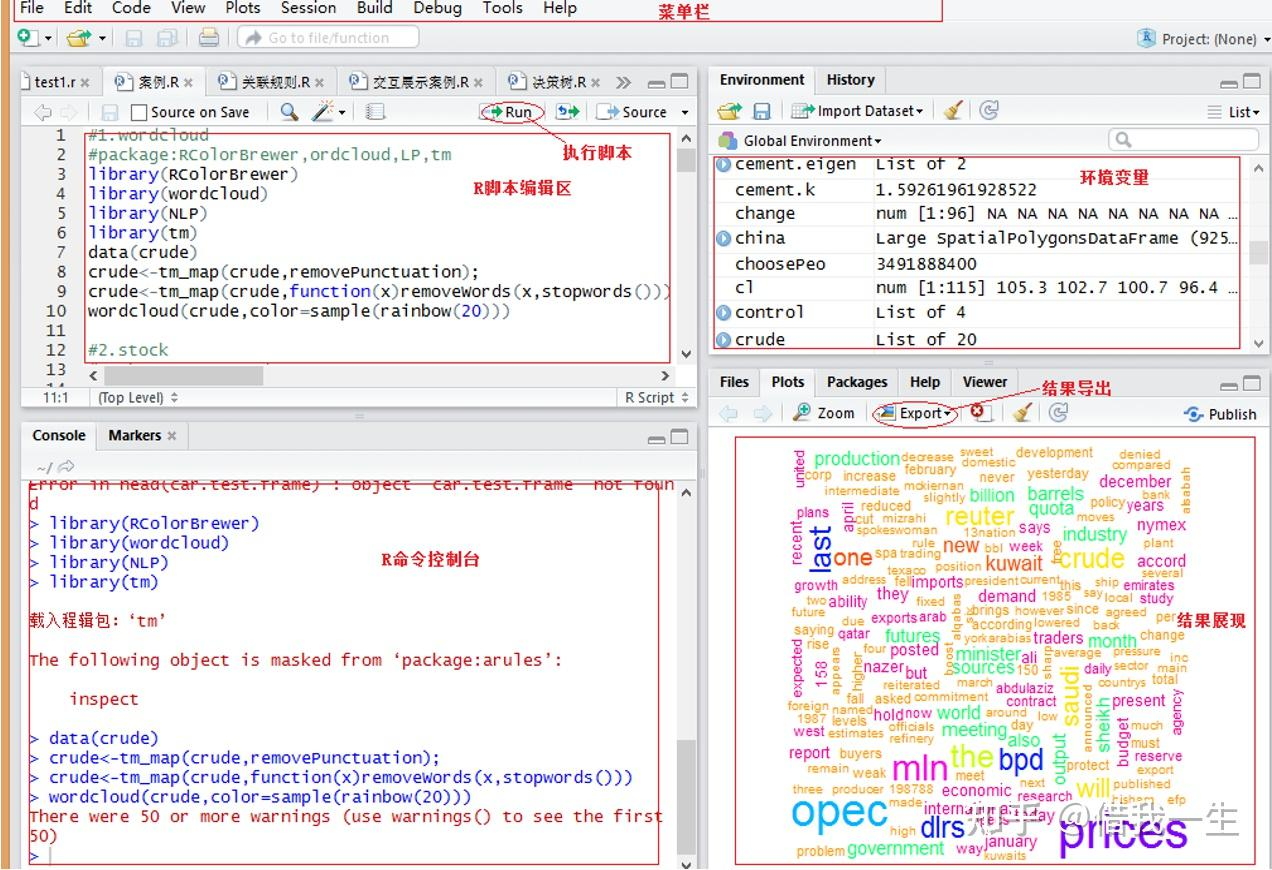
\includegraphics[width=1.0\textwidth]{Figure/Rstudio操作界面.jpg}
    \caption{R studio操作界面}
\end{figure}
\section{一个简单的示例(不是Hello World)}
\begin{lstlisting}[language=R, basicstyle=\ttfamily\small, backgroundcolor=\color{gray!10}, frame=leftline, xleftmargin=2em]
    # Listing 1.1 - A Sample R session
age <- c(1,3,5,2,11,9,3,9,12,3)
weight <- c(4.4,5.3,7.2,5.2,8.5,7.3,6.0,10.4,10.2,6.1)
mean(weight)
sd(weight)
cor(age,weight)
plot(age,weight)

\end{lstlisting}

